\chapter{Метрические методы анализа временных рядов}
\label{ch:metric_learning}

При использовании в качестве функции ошибки модели квадратичной ошибки предполагается, что целевое пространство является евклидовым. 
Данное предположение не всегда является адекватным.
В данной главе ставится задача метрического обучения как поиск оптимальной метрики в целевом пространстве.
Рассматриваются задачи кластеризации и классификации множества временных рядов.

%%%%%%%%%%%%%%%%%%%%%%%%%%%%%%%%%%%%%%%%%%%%%%%%
\section{Метрическое обучение в задачах кластеризации временных рядов}
\label{sec:ch5:metric_learning_clustering}
%%%%%%%%%%%%%%%%%%%%%%%%%%%%%%%%%%%%%%%%%%%%%%%%

Пусть~$\bX = [\bx_1, \dots, \bx_m]^{\T} \in \mathbb{R}^{m \times n}$~--- матрица исходных объектов.
Исходный объект~$\bx_i = [x_i^1, \ldots, x_i^n]^{\T}$ задан в виде вектора в пространстве признаков.
Требуется выявить кластерную структуру данных и разбить множество объектов~$\bX$ на множество непересекающихся кластеров $\bbY = \{1, \dots, K\}$, т.\,е.\ построить отображение $f: \bbR^n \to \bbY$.
Обозначим~$y_i = f (\bx_i)$, $y_i \in \bbY$~--- метка кластера объекта~$\bx_i$.
Необходимо выбрать метки кластеров~$\{y_i\}_{i=1}^m$ таким образом, чтобы расстояния между кластерами были максимальными.
Центроид~$\bmu$ множества объектов~$\bX$ и центроиды кластеров $\{\bmu_j\}_{j=1}^K$ вычисляются по формулам:
\begin{equation}
	\label{ch5:eq:mu}
	\boldsymbol{\mu} =\frac{1}{m} \sum_{i=1}^m\bx_i, \quad
	\boldsymbol{\mu}_j =\frac{ \sum_{i=1}^m [y_i = y_j]\bx_i } {\sum_{i=1}^m [y_i = y_j]}\,.
\end{equation}
Введем на множестве объектов~$\bX$ расстояние Махаланобиса
\begin{equation}
	d_{\bA} (\bx_i, \bx_j) = \sqrt{(\bx_i - \bx_j)^{\top} \bA^{-1} (\bx_i - \bx_j)},
	\label{ch5:eq:mahal_distance}
\end{equation}
где \textit{матрица трансформаций} $\mathbf{A} \in \bbR^{n \times n}$ является симметричной и неотрицательно определенной ($\mathbf{A}^{\T} = \mathbf{A}$, $\mathbf{A} \succeq 0$).
Зададим в качестве матрицы трансформации матрицу выборочной ковариации
\begin{equation}
	\label{ch5:eq:covMatrix}
	\bA = \frac{1}{m} \sum_{i=1}^m(\bx_i - \bmu)(\bx_i - \bmu)^{\T}.
\end{equation}
Функцией ошибки кластеризации назовем межкластерное расстояние:
\begin{equation}
	\cL \bigl(\{\bmu_j\}_{j=1}^K, \bX, \by\bigr)= - \sum_{j=1}^K N_j d_{\bA}^2(\bmu_j, \bmu),
	\label{ch5:eq:cluster_error_function}
\end{equation}
где $N_j = \sum_{i=1}^m [y_i = y_j]$~--- число объектов в кластере~$j$.

Поставим задачу кластеризации как задачу минимизации функции ошибки~\eqref{ch5:eq:cluster_error_function}
\begin{equation}
	\label{ch5:eq:Qmax}
	\cL \bigl(\{\boldsymbol{\mu}_j\}_{j=1}^K, \bX, \by \bigr) \to \min_{\boldsymbol{\mu}_j \in \bbR^{\T}}.
\end{equation}
Для решения этой задачи предлагается применить метод метрического обучения к матрице трансформации~$\bA$.
Найдем такую матрицу~$\bA$, для которой функционал качества принимает максимальное значение:
\begin{equation}
	\label{ch5:eq:Amax}
	\bA^* =\argmin_{\bA \in \bbR^{n \times n}} S \bigl(\{\bmu_j^*\}_{j=1}^K, \bX, \by \bigr)\,,
\end{equation}
где $\{\bmu_j^*\}_{j=1}^K$~--- решение задачи кластеризации~\eqref{ch5:eq:Qmax}.

%%%%%%%%%%%%%%%%%%%%%%%%%%%%%%%%%%%%%%%%%%%%%%%%
\section{Алгоритм адаптивного метрического обучения}
\label{sec:ch5:metric_learning_adaptive}
%%%%%%%%%%%%%%%%%%%%%%%%%%%%%%%%%%%%%%%%%%%%%%%%

Для решения задач~\eqref{ch5:eq:Qmax}, \eqref{ch5:eq:Amax} используется алгоритм адаптивного метрического обучения.
Предлагается понизить размерность пространства объектов~$\bX$ с помощью линейного ортогонального преобразования~$\bP \in \bbR^{l \times n}$, $\bP^{\T} \bP = \mathbf{I}$, где новая размерность $l < n$
\[
	\bt_i = \bP \bx_i \in \bbR^l, \quad i = 1, \dots, m.
\]
Центроид~$\hat{\bmu}$ множества объектов~$\{\bt_i\}_{i=1}^m$ вычисляется по формуле~\eqref{ch5:eq:mu}. 
Расстояния между объектами вычисляются по формуле~\eqref{ch5:eq:mahal_distance}, где в качестве матрицы~$\hat{\mathbf{A}}$ используется матрица ковариаций~\eqref{ch5:eq:covMatrix} множества объектов $\{\hat{\bx}_i\}_{i=1}^m$
\[
	\hat{\mathbf{A}} =
	\frac{1}{m} \sum_{i=1}^m (\bt_i - \hat{\bmu})(\bt_i - \hat{\bmu})^{\T} =
	\frac{1}{m} \sum_{i=1}^m \bP(\bx_i - \bmu)(\bx_i - \bmu)^{\T} \bP^{\T} =  \bP \mathbf{A} \bP^{\T}.
\]
\begin{definition}
	\textit{Индикаторной матрицей} назовем матрицу $\bY \in \bbR^{m \times K}$, где
	$y_{ij} =[f(\bx_i) = y_j]$.
\end{definition}
\begin{definition}
	\textit{Взвешенной индикаторной матрицей} назовем матрицу
	$\mathbf{L} = \bY (\bY^{\T} \bY)^{-1/2} \in \bbR^{m \times K}$, элементы которой равны:
	\[
		l_{ij} =
		\begin{cases}
			\displaystyle    \frac{1}{\sqrt{N_j}}, & \text{если $f(\bx_i) = y_j$;} \\
			0, & \text{если $f(\bx_i) \neq y_j$.}
		\end{cases}
	\]
\end{definition}
В работе~\cite{ding2005equivalence} показано, что с использованием данных обозначений задача кластеризации~\eqref{ch5:eq:Qmax} и~задача метрического обучения~\eqref{ch5:eq:Amax} сводятся к общей задаче минимизации функции ошибки
\begin{multline}
	\cL = -\frac{1}{m} \text{trace} (\mathbf{L}^{\T} \bX^{\T} \bP^{\T} \hat{\mathbf{A}}^{-1} \bP \bX \mathbf{L}) = \\ = - \frac{1}{m} \text{trace} (\mathbf{L}^{\T} \bX^{\T} \bP^{\T}
	(\bP \mathbf{A} \bP^{\T})^{-1} \bP \bX \mathbf{L}) \to \min_{\bP, \mathbf{L}}.
	\label{ch5:eq:GLmax}
\end{multline}

Для решения задачи~\eqref{ch5:eq:GLmax} используется EM алгоритм.
На каждом шаге итеративно вычисляются текущие оптимальные значения матриц~$\bP$ и~$\mathbf{L}$.
На $E$-шаге необходимо найти матрицу~$\mathbf{L}$, которая является решением оптимизационной задачи~\eqref{ch5:eq:GLmax} при фиксированной матрице~$\bP$.
В качестве начального приближения получим взвешенную индикаторную матрицу~$\mathbf{L}$ с помощью алгоритма кластеризации $k$-средних с евклидовой метрикой.
На $M$-шаге производится нахождение оптимального значения матрицы~$\bP$ при фиксированной матрице~$\mathbf{L}$.
Алгоритм завершается при стабилизации функционала~$\cL$ на последовательности итераций.

\textbf{Алгоритм $k$-средних.}
В данной работе базовым алгоритмом для сравнения является алгоритм $k$-средних.
На первом шаге алгоритм выбирает из множества~$\bX$ случайным образом~$r$ объектов~$\{\bmu_j\}_{j=1}^K$~--- начальные центроиды кластеров.
Для каждого объекта~$\bx_i$ вычисляется расстояние~\eqref{ch5:eq:mahal_distance} до каждого центроида кластера~$\bmu_j$ с единичной матрицей трансформаций~$\mathbf{A}$.
Объект~$\bx_i$ относится к кластеру, расстояние до которого оказалось наименьшим.
Далее производится вычисление новых центроидов кластеров по формуле~\eqref{ch5:eq:mu}.
Алгоритм завершается, если значения центроидов кластеров стабилизируются.

\textbf{Оптимизация матрицы P с фиксированной матрицей L.}
Для любых двух квадратных матриц~$\mathbf{A}$ и~$\mathbf{B}$ справедливо $\text{trace}(\mathbf{AB}) = \text{trace}(\mathbf{BA})$.
Данное свойство позволяет переформулировать задачу~\eqref{ch5:eq:GLmax} следующим образом:
\[
	\cL = -\frac{1}{m} \text{trace} (\mathbf{L}^{\T} \bX^{\T} \bP^{\T} (\bP \mathbf{A} \bP^{\T})^{-1} \bP \bX \mathbf{L}) = -\frac{1}{m} \text{trace} \bigl((\bP \mathbf{A} \bP^{\T})^{-1} \bP \bX \mathbf{LL}^{T} \bX^{\T} \bP^{\T}\bigr).
\]
\begin{statement}
	Обозначим $\mathbf{B} = \bX \mathbf{LL}^{\T} \bX^{\T}$.
	Обозначим через $\bP = [\mathbf{v}_1, \ldots, \mathbf{v}_r]^{\bT}$ матрицу, состоящую из $r$ собственных векторов матрицы $\mathbf{A}^{-1}\mathbf{B}$, отвечающих наибольшим собственным значениям.
	Тогда решением~\eqref{ch5:eq:GLmax} является ортогональная матрица, полученная QR-разложением матрицы~$\bP^{\T}$.
\end{statement}
\begin{proof}
Функция ошибки~$\cL$~\ref{ch5:eq:cluster_error_function} зависит только от матрицы~$\bP$. Обозначим
\[
	s(\bP) = \text{trace} \bigl((\bP \mathbf{A} \bP^{\T})^{-1} \bP \mathbf{B} \bP^{\T}\bigr).
\]
На данном шаге задача~\eqref{ch5:eq:GLmax} принимает вид:
\begin{gather}
	\label{ch5:eq:Gmax}
	\bP^* = \argmax_{\bP \in \bbR^{l \times n}} s(\bP)\,; \\
	\label{ch5:eq:Gorth}
	\bP \bP^{\T} = \mathbf{I}\,.
\end{gather}
Ранг произведения матриц не превосходит рангов сомножителей, поэтому ранг матрицы~$\mathbf{B}$ не превосходит $K$.
Решением~\eqref{ch5:eq:Gmax} является матрица $\bP = [\mathbf{v}_1, \ldots, \mathbf{v}_K]^{\T}$, состоящая
из~$K$ собственных векторов матрицы $\mathbf{A}^{-1}\mathbf{B}$, отвечающих наибольшим собственным значениям.
Таким образом, размерность нового пространства объектов будет равна количеству кластеров $K$.

В общем случае матрица $\bP$ не является ортогональной.
Заметим, что для любой невырожденной матрицы $\bP$ верно $s(\bP) = s(\mathbf{M} \bP)$.
Для учета условия ортогональности~\eqref{ch5:eq:Gorth} найдем QR-разложение матрицы $\bP$.
Тогда ортогональная матрица $\bQ$ является оптимальным значением $\bP^*$.
\end{proof}

\textbf{Оптимизация матрицы L с фиксированной матрицей P.}
Обозначим $\hat{\mathbf{K}} = (1/N)\bX^{\T} \bP^{\T} \hat{\mathbf{A}}^{-1} \bP \bX$.
В работе~\cite{shawe2004kernel} показано, что тогда задача~\eqref{ch5:eq:GLmax} эквивалентна задаче кластеризации $k$-средних с заданным ядром $\hat{\mathbf{K}}$.

При фиксированной матрице $\bP$ задача~\eqref{ch5:eq:GLmax} принимает вид:
\begin{equation*}
	\text{trace} (\mathbf{L}^{\top} \hat{\mathbf{K}} \mathbf{L}) \to \max_{\mathbf{L} \in \bR^{m \times r}}.
\end{equation*}
Матрица $\hat{\mathbf{K}}$ является симметричной и неотрицательно определенной, тем самым может быть выбрана в качестве ядра.

%%%%%%%%%%%%%%%%%%%%%%%%%%%%%%%%%%%%%%%%%%%%%%%%
\section{Задача метрического обучения с динамическим выравниваем временных рядов}
\label{sec:ch5:metric_learning_classification}
%%%%%%%%%%%%%%%%%%%%%%%%%%%%%%%%%%%%%%%%%%%%%%%%

Пусть объект $\mathbf{x}_i \in \mathbb{R}^n$~--- временной ряд, последовательность измерений некоторой исследуемой величины в различные моменты времени.
Пусть задана выборка $\{(\mathbf{x}_i, y_i)\}_{i=1}^m$~--- множество объектов с известными метками классов $y_i \in \bbY$, где $\bbY = \{1, \dots, K\}$~--- множество меток классов.

Требуется построить точную, простую, устойчивую модель классификации $a: \bbR^n \to \bbY$.
Данную модель представим в виде суперпозиции
\begin{equation*}
	a(\mathbf{x}) = b \circ \mathbf{f} \circ G\bigl(\mathbf{x}, \{\mathbf{c}_e\}_{e = 1} ^ K\bigr),
\end{equation*}
где $G$~--- процедура выравнивания временных рядов относительно центроидов классов~$\{\mathbf{c}_e\}_{e = 1} ^ K$, $\mathbf{f}$~--- алгоритм метрического обучения, $b$~--- алгоритм многоклассовой классификации.

\textbf{Выравнивание временных рядов.}
Для повышения качества и устойчивости алгоритма классификации предлагается провести выравнивание временных рядов каждого класса относительно центроида.

\begin{definition}
	\textit{Центроидом} множества объектов $\bX_e$ по расстоянию $\rho$ назовем вектор $\mathbf{c}_e \in \mathbb{R}^n$ такой, что
	\begin{equation}
		\label{ch5:eq:centroid_task}
		\mathbf{c}_e = \mathop{\text{argmin}}\limits_{{\mathbf{c} \in \mathbb{R}^n}}\sum_{\mathbf{x}_i \in \mathbf{X}_e}
		{\rho(\mathbf{x}_i ,\mathbf{c})}.
	\end{equation}
	Здесь $\bX_e = \{\bx_i: i=1, \dots, m, \, y_i=e\}$~--- множество объектов выборки, принадлежащих одному классу $e \in \bbY$.
\end{definition}

Для нахождения центроида предлагается в качестве расстояния между временными рядами использовать путь наименьшей стоимости~\cite{berndt1994using,muller2007dynamic}, найденный методом динамической трансформации времени.
Псевдокод решения оптимизационной задачи~\eqref{ch5:eq:centroid_task} приведен в алгоритме~\ref{ch5:alg:DBA_pseudo}.
\begin{algorithm}[!t]
	\caption{Нахождение центроида $\text{DBA}(\mathbf{X}_e, \text{n\_iter})$}
	\label{ch5:alg:DBA_pseudo}
	\begin{algorithmic}[1]
		\REQUIRE $\mathbf{X}_e$~--- множество временных рядов, принадлежащих одному и тому же классу, n\_iter~--- количество итераций алгоритма.
		\ENSURE $\mathbf{c}$~--- центроид множества $\mathbf{X}_e$.
		
		\STATE {задать начальное приближение приближение центроида $\mathbf{c}$;}
		\FOR {$i = 1, \dots, \text{n\_iter}$}
		\FOR {$\mathbf{x} \in \mathbf{X}_e$}
		\STATE{вычислить выравнивающий путь между $\mathbf{c}$ и $\mathbf{x}$}
		\STATEx $ \quad \quad \text{alignment}(\mathbf{x}) := \text{DTWalignment}(\mathbf{c}, \mathbf{x})$;
		\ENDFOR
		\STATE {объединить поэлементно множества индексов для каждого отсчета времени}
		\STATEx {$ \quad \text{alignment} := \bigcup_{\mathbf{x} \in \mathbf{X}_e} \text{alignment}(\mathbf{x})$};
		\STATE {$\mathbf{c} = \text{mean}(\text{alignment})$}
		\ENDFOR
	\end{algorithmic}

	\textbf{DTWalignment}($\mathbf{c}$, $\mathbf{x}$)
	\begin{algorithmic}[1]
		\REQUIRE $\mathbf{c}, \mathbf{x}$~--- временные ряды.
		\ENSURE alignment~--- выравнивающий путь.\COMMENT {каждый индекс временного ряда~$\mathbf{x}$ поставлен в однозначное соответствие индексу временного ряда~$\mathbf{c}$}
		
		\STATE {построить $n \times n$-матрицу деформаций DTW}
		\STATEx {$\text{cost} := \text{DTW}(\mathbf{c}, \mathbf{x})$};
		
		\STATE {вычислить выравнивающий путь по матрице деформаций}
		\STATEx {$\text{alignment} := \text{DTWpath}(\text{cost})$};
	\end{algorithmic}
\end{algorithm}
Общая процедура выравнивания имеет следующий вид:
\begin{itemize}
	\item[1)]
	построить множество центроидов классов $\{\mathbf{c}_e\}_{e = 1}^K$;
	\item[2)]
	по множеству центроидов найти пути наименьшей стоимости между каждым
	временным рядом $\mathbf{x}_i$ и центроидом его класса $\mathbf{c}_{y_i}$;
	\item[3)]
	по каждому пути восстановить выравненный временной ряд;
	\item[4)]
	привести множества выравненных временных рядов к нулевому среднему и нормировать на дисперсию.
\end{itemize}

Результатом выравнивания должно стать множество выравненных временных рядов.

\textbf{Метрическое обучение.}
Введем на множестве выравненных временных рядов расстояние Махаланобиса $d_{\bA}$~\ref{ch5:eq:mahal_distance}.
Представим матрицу трансформации~$\bA$ в виде разложения $\mathbf{A}^{-1} = \mathbf{L}^{\T}  \mathbf{L}$.
Матрица $\mathbf{L} \in \bbR^{p \times n}$~--- матрица линейного преобразования, где $p$ задает размерность преобразованного пространства. Если параметр $p < n$, то происходит снижение размерности признакового пространства.

Расстояние $d_\mathbf{A} (\mathbf{x}_i, \mathbf{x}_j)$ есть евклидово расстояние между $\mathbf{Lx}_i$ и $\mathbf{Lx}_j$:
\begin{multline*}
	d_\mathbf{A} (\mathbf{x}_i, \mathbf{x}_j) = \sqrt{(\mathbf{x}_i - \mathbf{x}_j)^{\T} \mathbf{L}^{\T} \mathbf{L} (\mathbf{x}_i - \mathbf{x}_j)} = \\= \sqrt{(\mathbf{L} (\mathbf{x}_i - \mathbf{x}_j))^{\T} (\mathbf{L} (\mathbf{x}_i - \mathbf{x}_j))} = \|\mathbf{L} (\mathbf{x}_i - \mathbf{x}_j)\|_2.
\end{multline*}

В качестве алгоритма метрического обучения в данной работе был выбран алгоритм LMNN~\cite{weinberger2009distance}. 
Данный алгоритм сочетает в себе идеи метода $k$ ближайших соседей. 
Первая идея заключается в минимизации расстояний между $k$ ближайшими объектами, находящимися в одном классе. 
Запишем функционал качества в виде
\[
	Q_1(\mathbf{L}) = \sum_{j \rightsquigarrow i} \|\mathbf{L}(\mathbf{x}_i - \mathbf{x}_j)\|^2 \rightarrow \min_{\mathbf{L}},
\]
где запись $j \rightsquigarrow i$ означает, что $\mathbf{x}_j$ является одним из $k$ ближайших соседей для $\mathbf{x}_i$.
Вторая идея состоит в максимизации расстояния между каждым объектом и его объектами-нарушителями. 

\begin{definition}
	\textit{Объектом-нарушителем} для $\mathbf{x}_i$ назовем объект~$\mathbf{x}_l$ такой, что
	\begin{equation}
		\label{ch5:eq:impostor}
		\|\mathbf{L}(\mathbf{x}_i - \mathbf{x}_l)\|^2 \leq \|\mathbf{L}(\mathbf{x}_i - \mathbf{x}_j)\|^2 + 1, \quad \text{где $j \rightsquigarrow i$}.
	\end{equation}
\end{definition}
Таким образом, необходимо минимизировать следующий функционал:
\[
	Q_2(\mathbf{L}) = \sum_{j \rightsquigarrow i} \sum_l [y_i \neq y_l] \bigl[1 + \|\mathbf{L}(\mathbf{x}_i - \mathbf{x}_j)\|^2 - \|\mathbf{L}(\mathbf{x}_i - \mathbf{x}_l)\|^2\bigr]_+ \rightarrow \min_{\mathbf{L}}.
\]
Положительная срезка позволяет штрафовать только те объекты, которые удовлетворяют условию~\eqref{ch5:eq:impostor}.

Задача метрического обучения состоит в нахождении линейного преобразования $\mathbf{f}(\mathbf{x}) = \mathbf{Lx}$, то есть нахождении матрицы $\mathbf{L}$ в виде решения оптимизационной задачи
\begin{equation}
	\label{ch5:eq:Qmin}
	Q(\mathbf{L}) = \mu Q_1(\mathbf{L}) + (1 - \mu) Q_2(\mathbf{L}) \rightarrow \min_{\mathbf{L}},
\end{equation}
где $\mu \in (0, 1)$~--- весовой параметр, определяющий вклад каждого из функционалов.
Задача~\eqref{ch5:eq:Qmin} представляет собой задачу полуопределенного программирования~\cite{vandenberghe1996semidefinite} и может быть решена существующими оптимизационными пакетами.

На Рис.~\ref{ch5:fig:metric_learning_toy_example} показан принцип работы алгоритма метрического обучения LMNN по сравнению с базовым методом, использующим евклидову метрику, для случая двумерных данных. 
Алгоритм LMNN позволяет найти оптимальную матрицу трансформации $\mathbf{A}$, отдаляя объекты разных классов и притягивая объекты одного класса. 
В случае использования евклидовой метрики матрица трансформаций $\mathbf{A}$ является единичной матрицей.

\begin{figure}[ht]
	\centering
	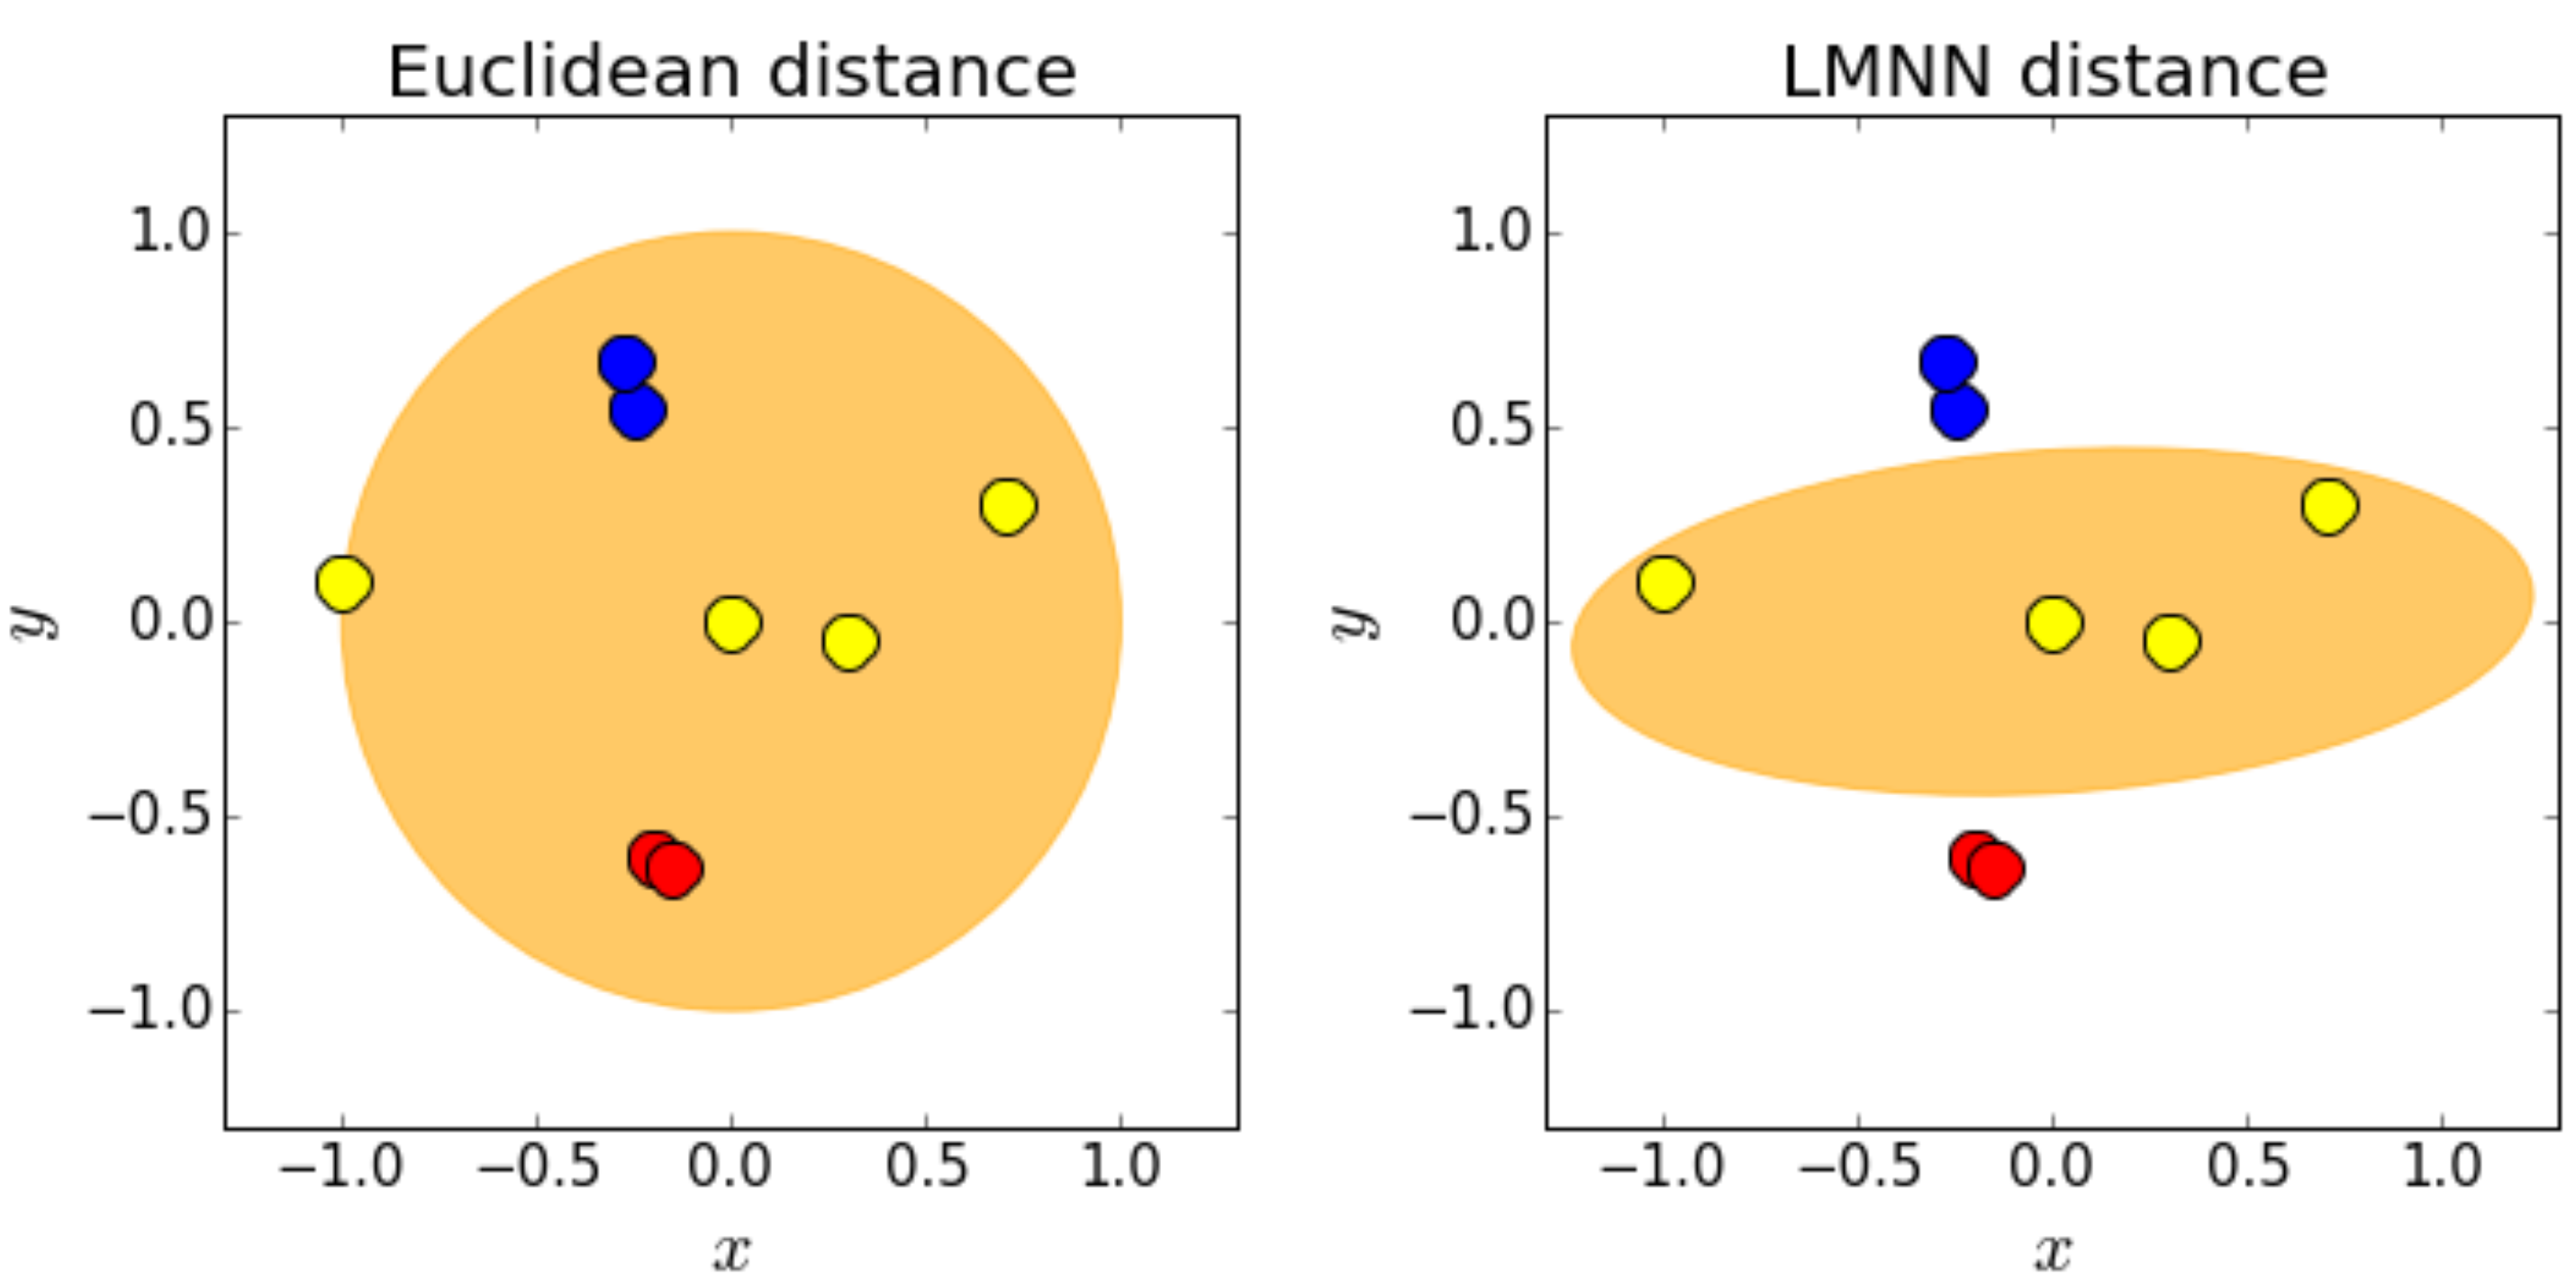
\includegraphics[width=0.9\linewidth]{figs/ch5/metric_learning_toy_example}
	\caption{Сравнение оптимальной метрики Махаланобиса алгоритма LMNN с евклидовой метрикой в двумерном случае}
	\label{ch5:fig:metric_learning_toy_example}
\end{figure}

\textbf{Классификация выравненных временных рядов в метрике Махаланобиса.}
Пусть $\mathbf{x} \in \mathbf{X}$~--- неразмеченный временной ряд. Выравниваем временной ряд $\mathbf{x}$ относительно всех центроидов классов
\[
	\mathbf{\hat{x}}_e = G(\mathbf{x}, \mathbf{c}_e), \quad \text{где} \quad e \in \{1, \dots, K\}.
\]
Отнесем временной ряд к классу, для которого минимально расстояние до соответствующего центроида. В качестве расстояния используем обученную метрику Махаланобиса с фиксированной матрицей $\mathbf{A}$
\[
	\hat{y} = \argmin_{e \in \bbY} d_\mathbf{A}(\mathbf{\hat{x}}_e, \mathbf{c}_e).
\]
После нахождения оптимальных центроидов классов и нахождения оптимальной матрицы трансформаций процедура классификации заключается в измерении расстояния между найденными центроидами и новыми неразмеченными объектами.

Для оценки качества работы алгоритма будем вычислять ошибку классификации как долю неправильно классифицированных объектов тестовой выборки~$\{ \bx_i, y_i \}_{i=1}^{\hat{m}}$:
\[
	\text{error} = \frac1{\hat{m}} \sum_{i = 1} ^ {\hat{m}} [a(\mathbf{x}_i) \ne y_i].
\]

%%%%%%%%%%%%%%%%%%%%%%%%%%%%%%%%%%%%%%%%%%%%%%%%
\section{Анализ метрического пространства для задачи кластеризации}
\label{sec:ch5:exp_clustering}
%%%%%%%%%%%%%%%%%%%%%%%%%%%%%%%%%%%%%%%%%%%%%%%%

В целях проверки работоспособности предложенного подхода проведен вычислительный эксперимент на модельных данных. Сгенерирована выборка объектов, принадлежащих одному из двух классов, в двумерном пространстве.
Каждый объект принадлежит многомерному нормальному распределению.
На Рис.~\ref{ch5:fig:true_distr} показано истинное распределение объектов, черным цветом выделены истинные центры классов и линии уровня функции распределения.

\begin{figure}[ht]
    \centering
    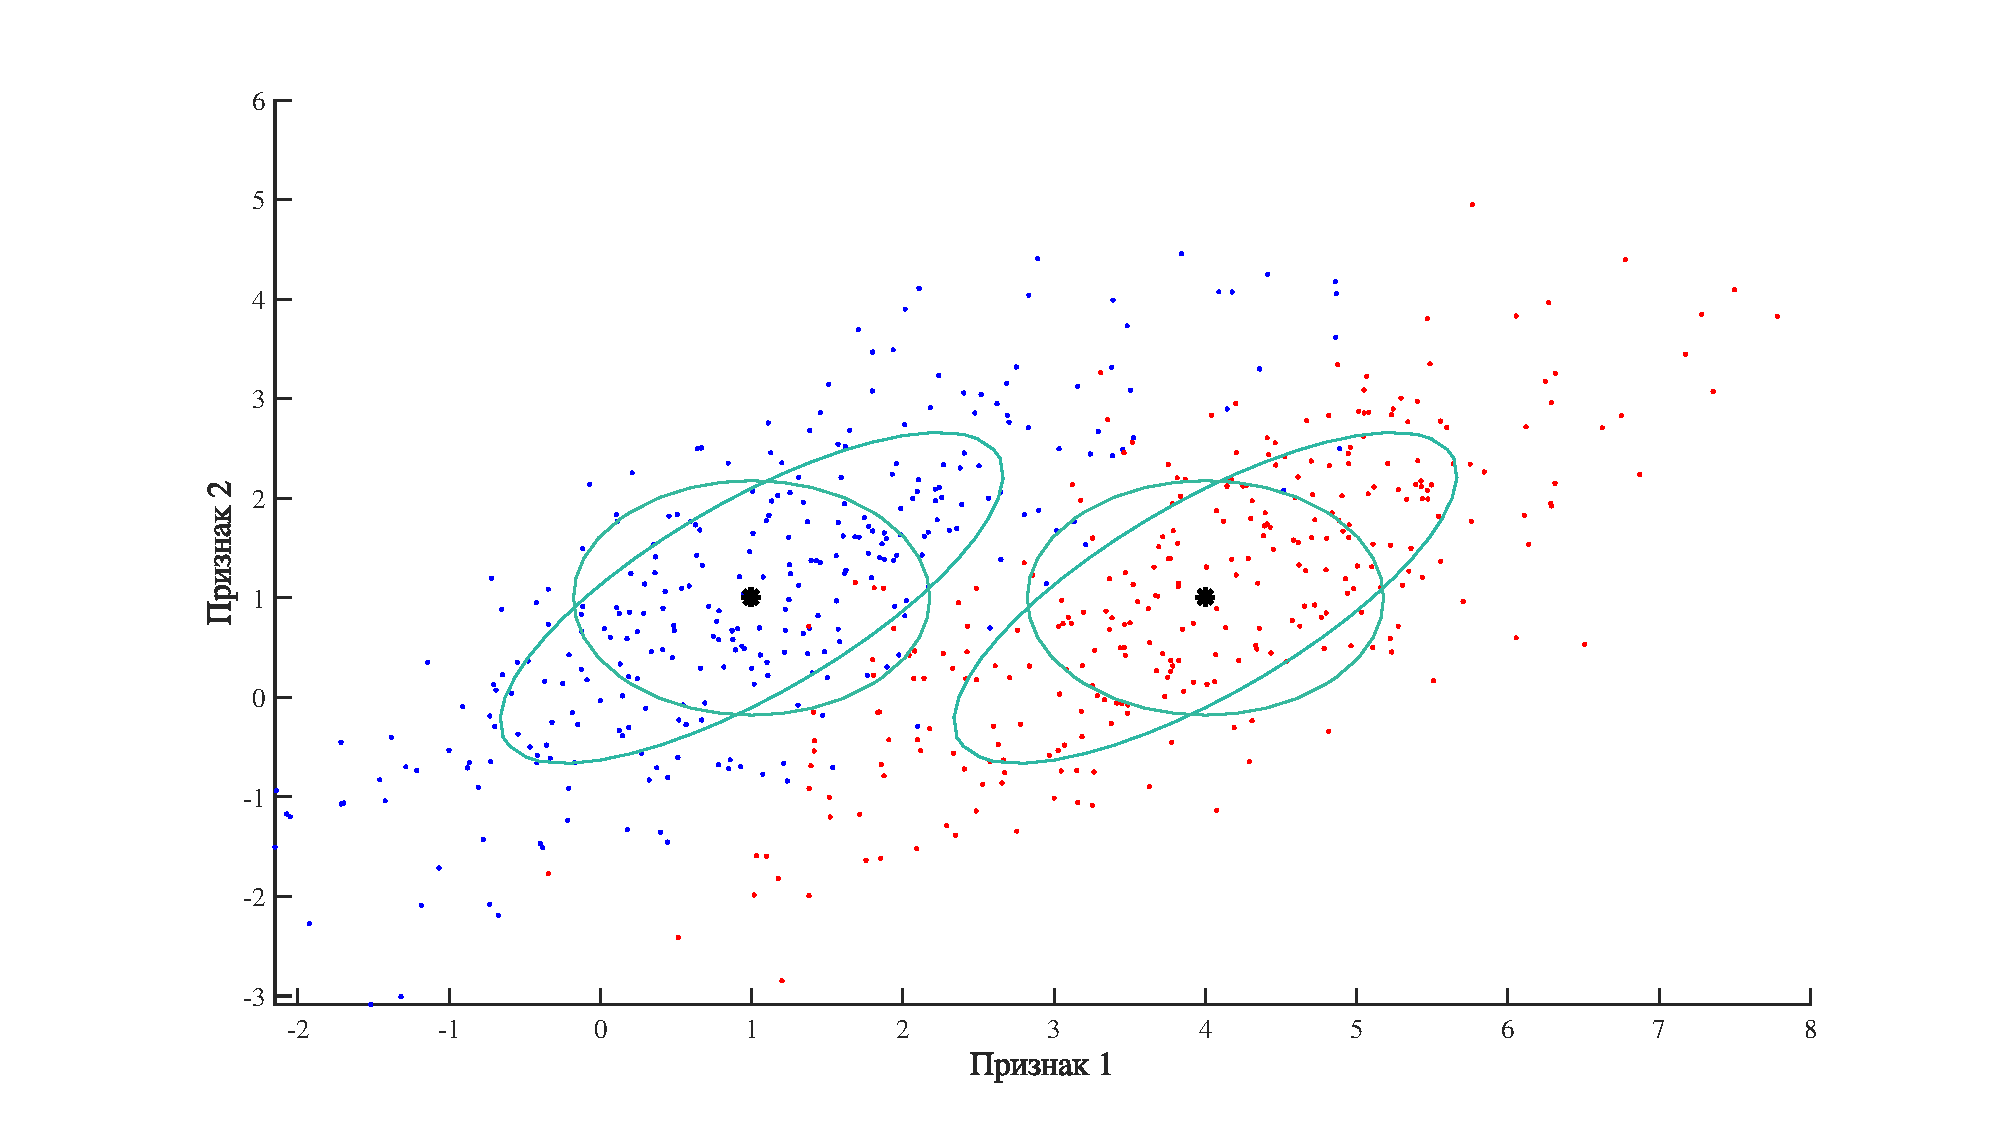
\includegraphics[width=\linewidth]{figs/ch5/true_distribution}
    \caption{Истинное распределение двумерных модельных данных}
    \label{ch5:fig:true_distr}
\end{figure}

Применим к данной выборке базовый алгоритм $k$-средних.
Результат кластеризации показан на Рис.~\ref{ch5:fig:kmeans_clustering}, где черным цветом выделены найденные центры классов и линии уровня функции распределения, построенной по выборочной матрице ковариаций.
\begin{figure}[ht]
    \centering
    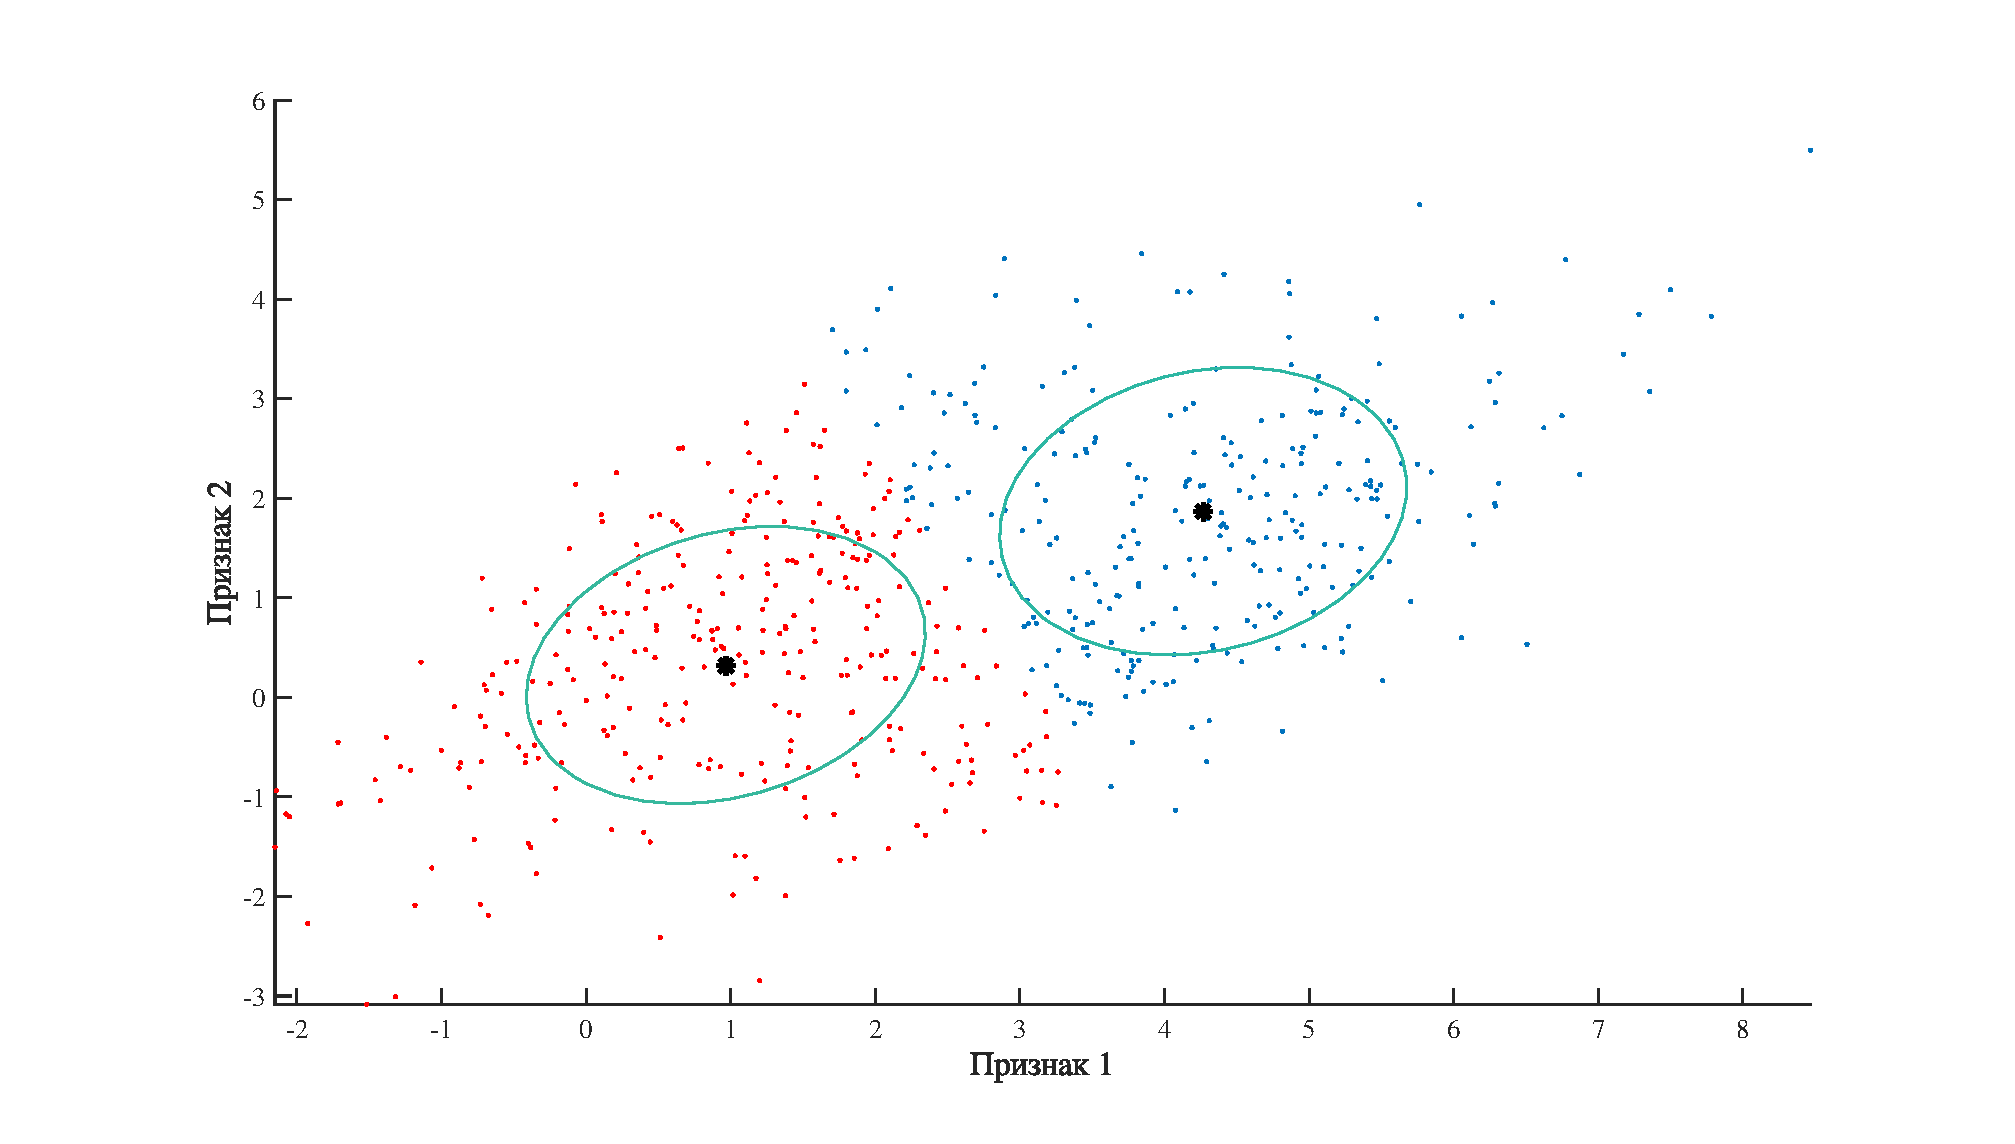
\includegraphics[width=1\linewidth]{figs/ch5/kmeans_clustering}
    \caption{Результат кластеризации модельных данных алгоритмом $k$-средних}
    \label{ch5:fig:kmeans_clustering}
\end{figure}
Взяв за начальное приближение результаты работы алгоритма $k$-средних,
проведем клас\-те\-ри\-за\-цию с помощью алгоритма адаптивного метрического обучения.
Результаты работы алгоритма продемонстрированы на Рис.~\ref{ch5:fig:AML_clustering}.

\begin{figure}[ht]
    \centering
    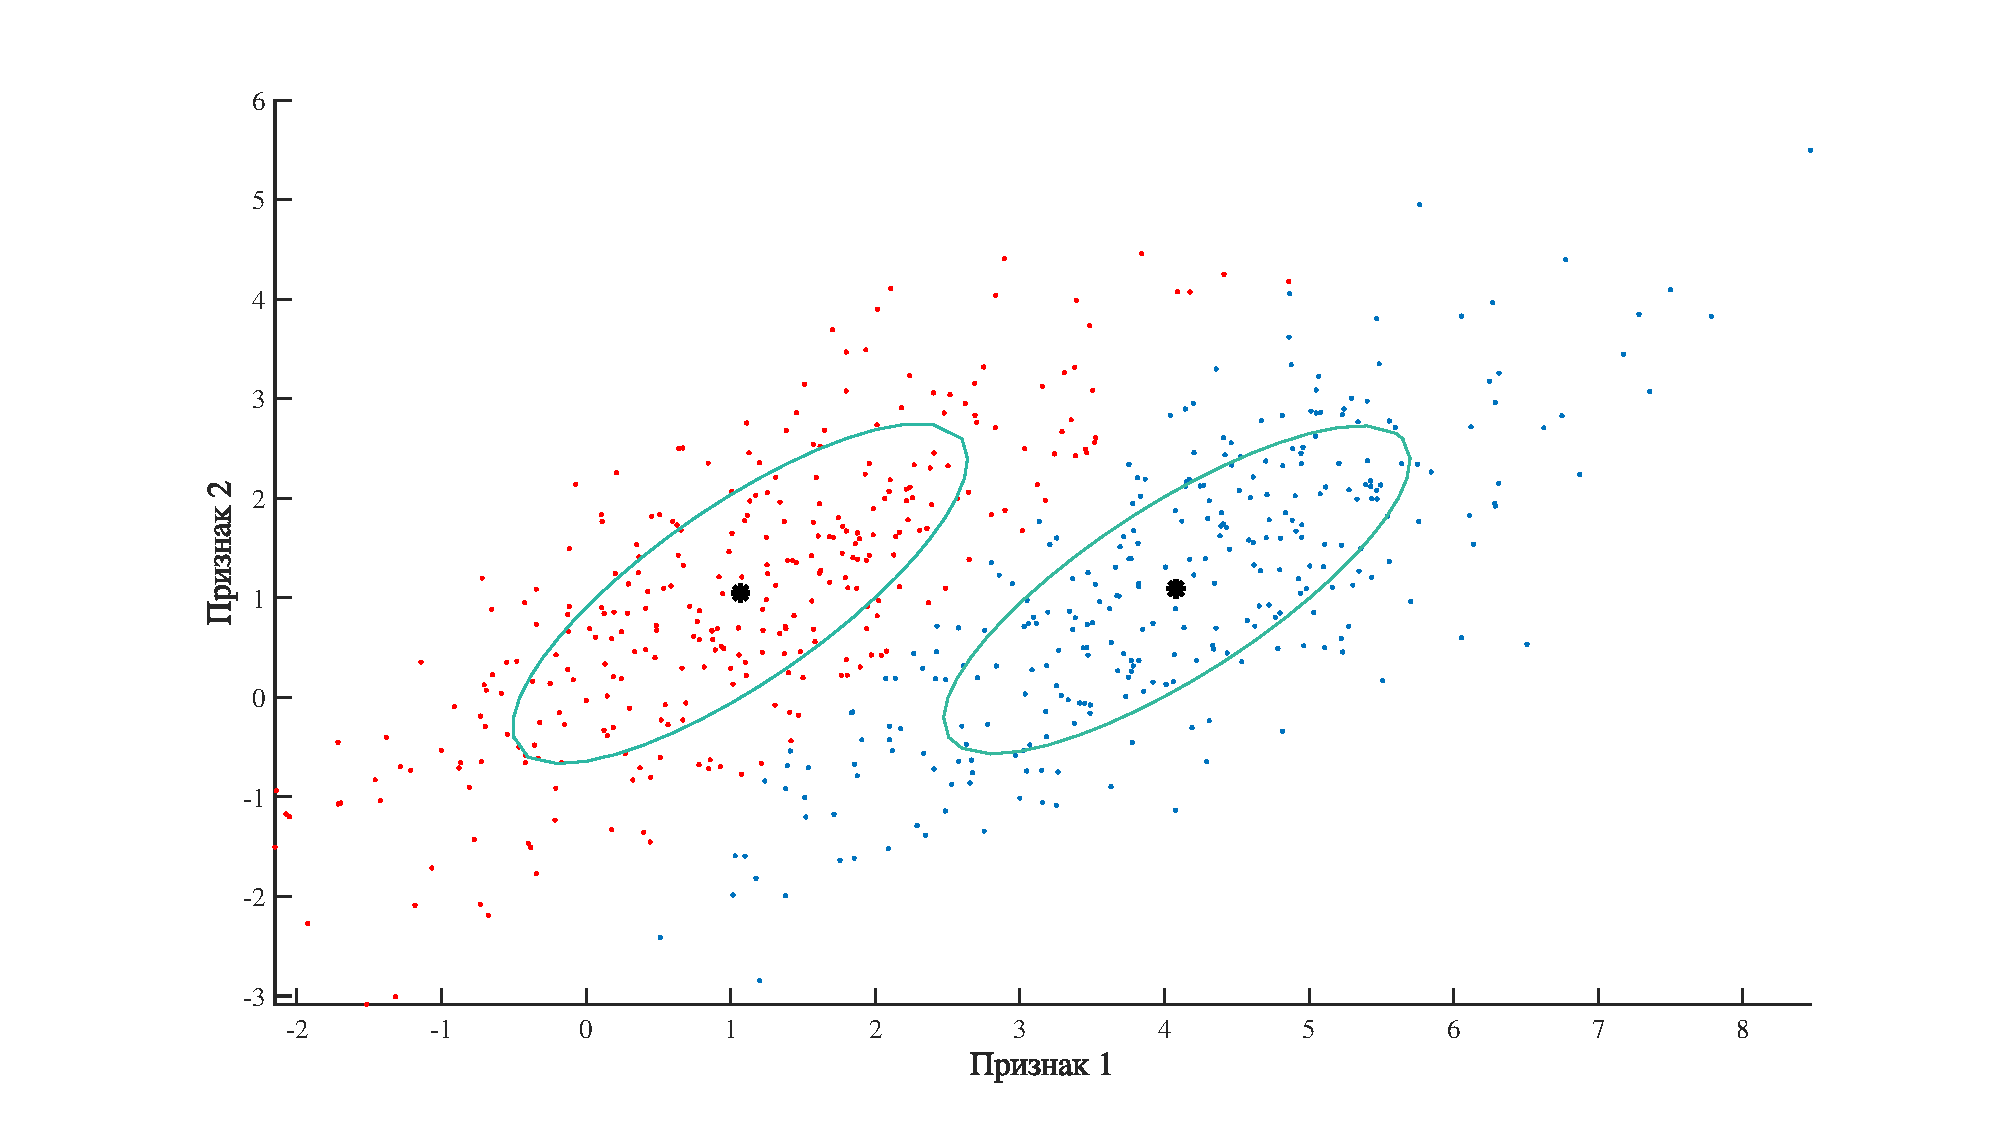
\includegraphics[width=1\linewidth]{figs/ch5/AML_clustering}
    \caption{Результат кластеризации модельных данных алгоритмом адаптивного метрического обучения}
    \label{ch5:fig:AML_clustering}
\end{figure}

На рисунках заметно улучшение результатов кластеризации.
Измеренная точность кластеризации алгоритма $k$-средних составила 0,76,
алгоритма адаптивного метрического обучения~--- 0,94, что говорит об эффективности данного подхода.

Таблица~\ref{ch5:tbl:clusteing_results} показывает результаты вычислительного эксперимента на реальных
данных.
Алгоритм был применен к $5$ выборкам, взятых из репозитория UCI~\cite{uci2017}.
Оценкой качества кластеризации служит число правильно кластеризованных объектов.
При кластеризации объектов на более чем два класса возникает проблема соотнесения истинных классов с полученными кластерами.
Данная проблема была формализована в виде задачи о назначениях и решена с помощью венгерского алгоритма. Вычислительный эксперимент на реальных данных показал увеличение точности кластеризации при использовании метрического обучения.
\begin{table}[!h]
\centering
\caption{Результаты кластеризации на множестве датасетов для методов $k$-средних и AML}
\label{ch5:tbl:clusteing_results}

\begin{tabular}{|l|l|l|}
\hline
\multicolumn{1}{|c}{Выборка}                  & \multicolumn{2}{|c|}{Качество кластеризации} \\ \cline{2-3}
                                          & $k$-средних               & AML                 \\
\hline
Letter Recognition                        & 0,356                 & \textbf{0,428}             \\
Optical Recognition of Handwritten Digits & 0,758                 & \textbf{0,790}               \\
Seeds                                     & 0,833                 & \textbf{0,881}            \\
Image Segmentation                        & 0,545                 & \textbf{0,737}            \\
Breast Cancer Wisconsin                   & \textbf{0,960}                 & 0,956               \\ \hline
\end{tabular}
\end{table}

%%%%%%%%%%%%%%%%%%%%%%%%%%%%%%%%%%%%%%%%%%%%%%%%
\section{Анализ метрического пространства для задачи классификации временных рядов}
\label{sec:ch5:exp_classification}
%%%%%%%%%%%%%%%%%%%%%%%%%%%%%%%%%%%%%%%%%%%%%%%%
	Цель вычислительного эксперимента~--- проверить работоспособность предложенного подхода.
	Предполагается, что построенный алгоритм мультиклассовой классификации способен определить тип активности человека по форме сигнала акселерометра мобильного телефона.
	
	Для проведения базового вычислительного эксперимента были подготовлены синтетические временные ряды, принадлежащие двум классам.
	Первый класс~--- синусы вида $sin(x + b)$, где параметр $b$ определяет сдвиг каждого временного ряда.
	Второй класс~--- пилообразные функции с различными сдвигами по временной шкале.
	На каждый временной ряд был наложен нормальный шум.
	Число временных рядов каждого класса = 60.
	Длина каждого временного ряда $n = 50$.
	
	Построенные центроиды классов проиллюстрированы на Рис.~\ref{ch5:fig:centroids_synthetic}.
	Из рисунка видно, что процедура корректно определяет сдвиги временных рядов.
	\begin{figure}[ht]
		\centering
		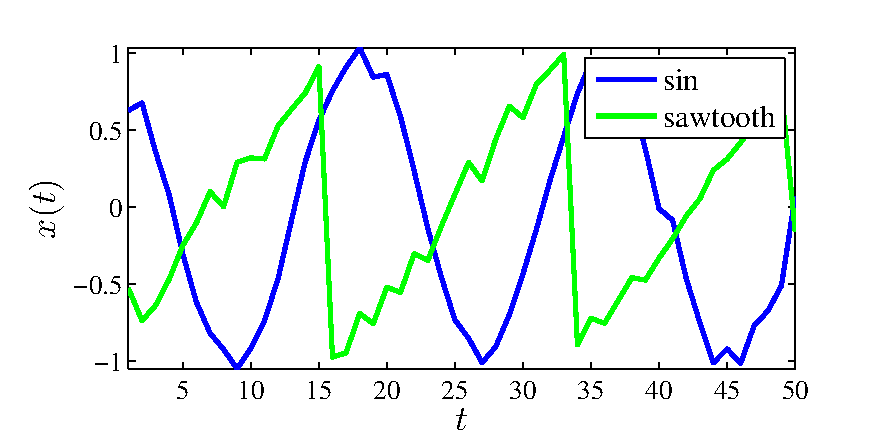
\includegraphics[width=0.5\linewidth]{figs/ch5/centroids_synthetic_noize}
		\caption{Примеры центроидов синтетических временных рядов}
		\label{ch5:fig:centroids_synthetic}
	\end{figure}
	
	Для того чтобы убедиться в целесообразности применения метрического обучения, данные
	временные ряды классифицировались в пространстве с евклидовой метрикой и в пространстве с метрикой Махаланобиса.
	Число ближайших соседей $k = 5$, размерность преобразованного пространства $p = 40$.
	Полученные ошибки классификации составили $27\%$ для евклидовой метрики и $6\%$ для метрики Махаланобиса.
	
	Реальные данные~\cite{wisdm} представляли собой временные ряды акселерометра мобильного телефона.
	Каждый из шести классов соответствовал определенной физической активности испытуемых.
	Для проведения вычислительного эксперимента было выбрано по $200$ объектов каждого класса.
	Длина каждого временного ряда равнялась $n = 128$ отсчетам времени.
	
	Построенные центроиды классов изображены на Рис.~\ref{ch5:fig:centroids_real}.
	Найденные центроиды обладают периодичностью, свойственной временным рядам показаний активности человека.
	\begin{figure}[ht]
		\centering
		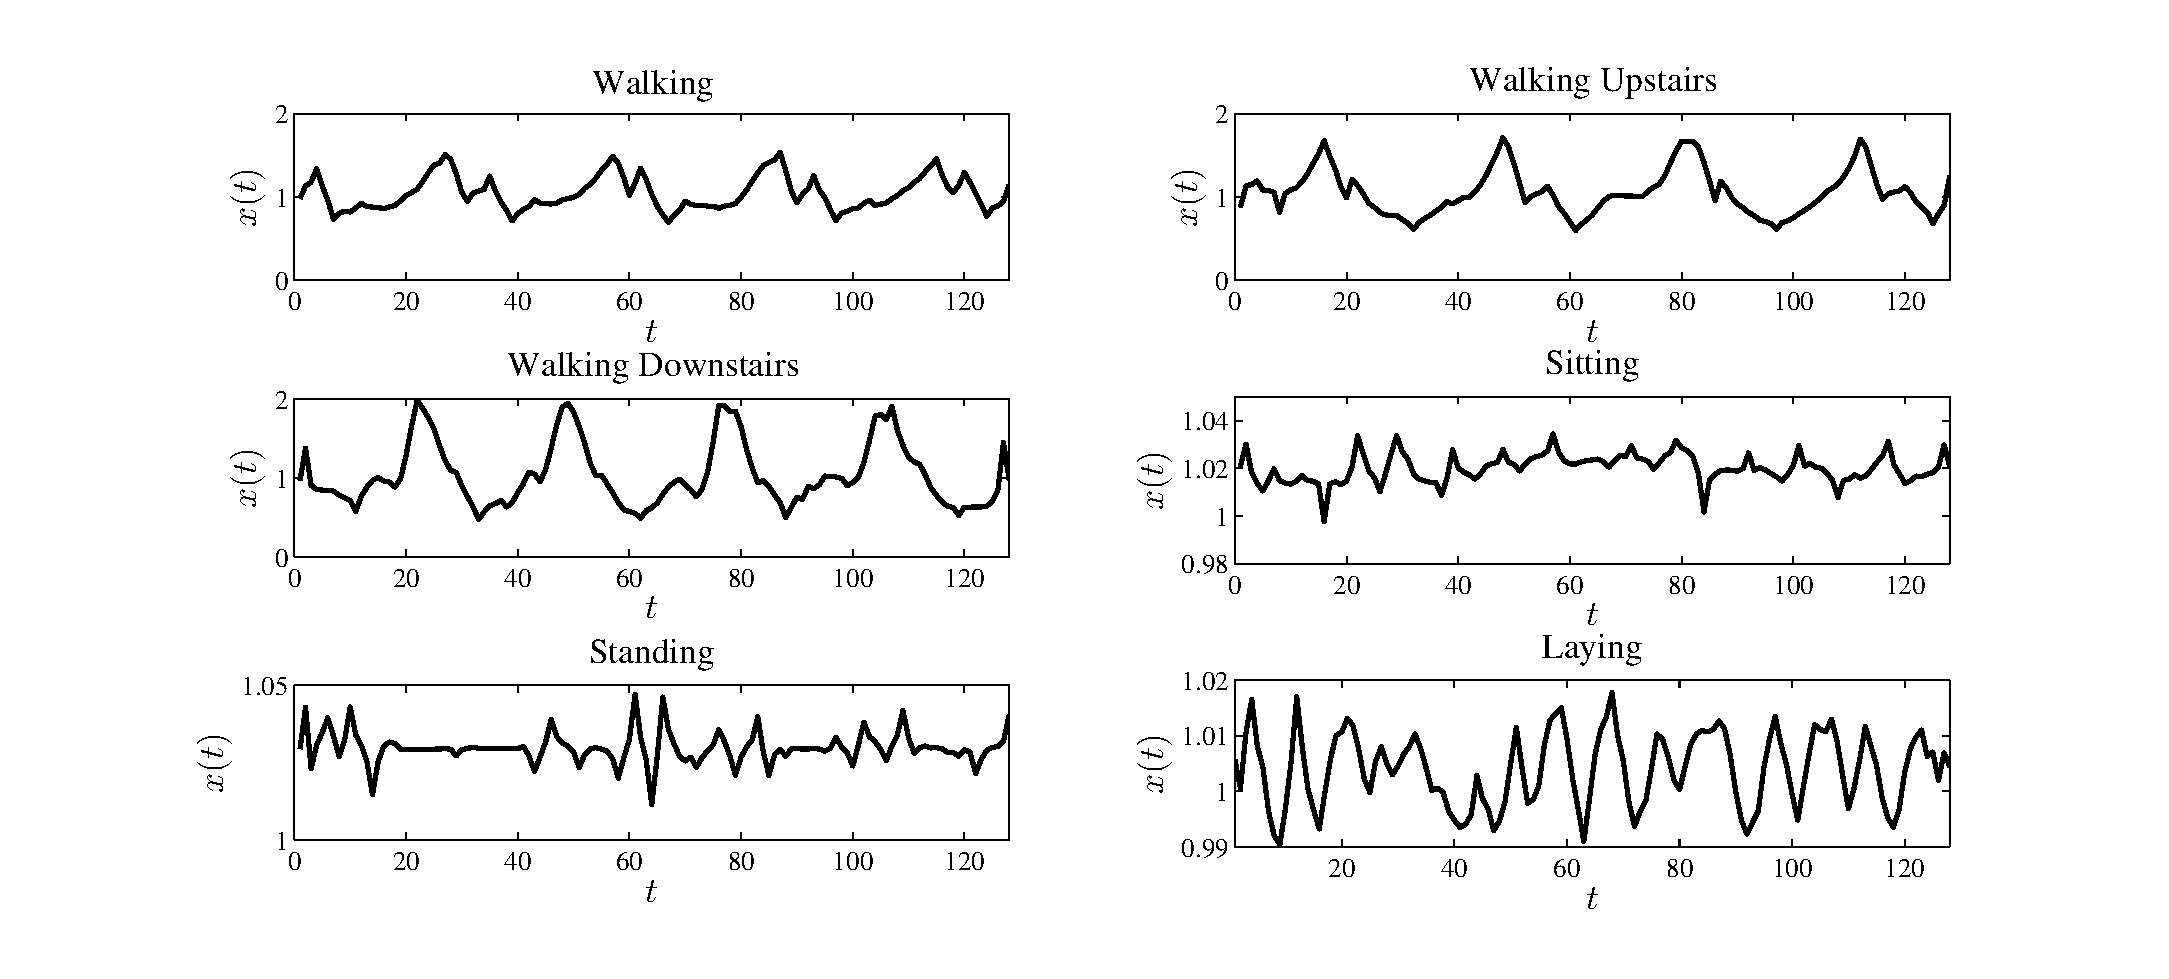
\includegraphics[width=1\linewidth]{figs/ch5/centroids_200_2}
		\caption{Примеры центроидов временных рядов акселерометра}
		\label{ch5:fig:centroids_real}
	\end{figure}
	На Рис.~\ref{ch5:fig:raw_ts} показаны примеры временных рядов каждого класса. Эти же временные ряды после процедуры выравнивания относительно построенных центроидов изображены на Рис.~\ref{ch5:fig:aligned_ts}.
	\begin{figure}[!ht]
		\centering
		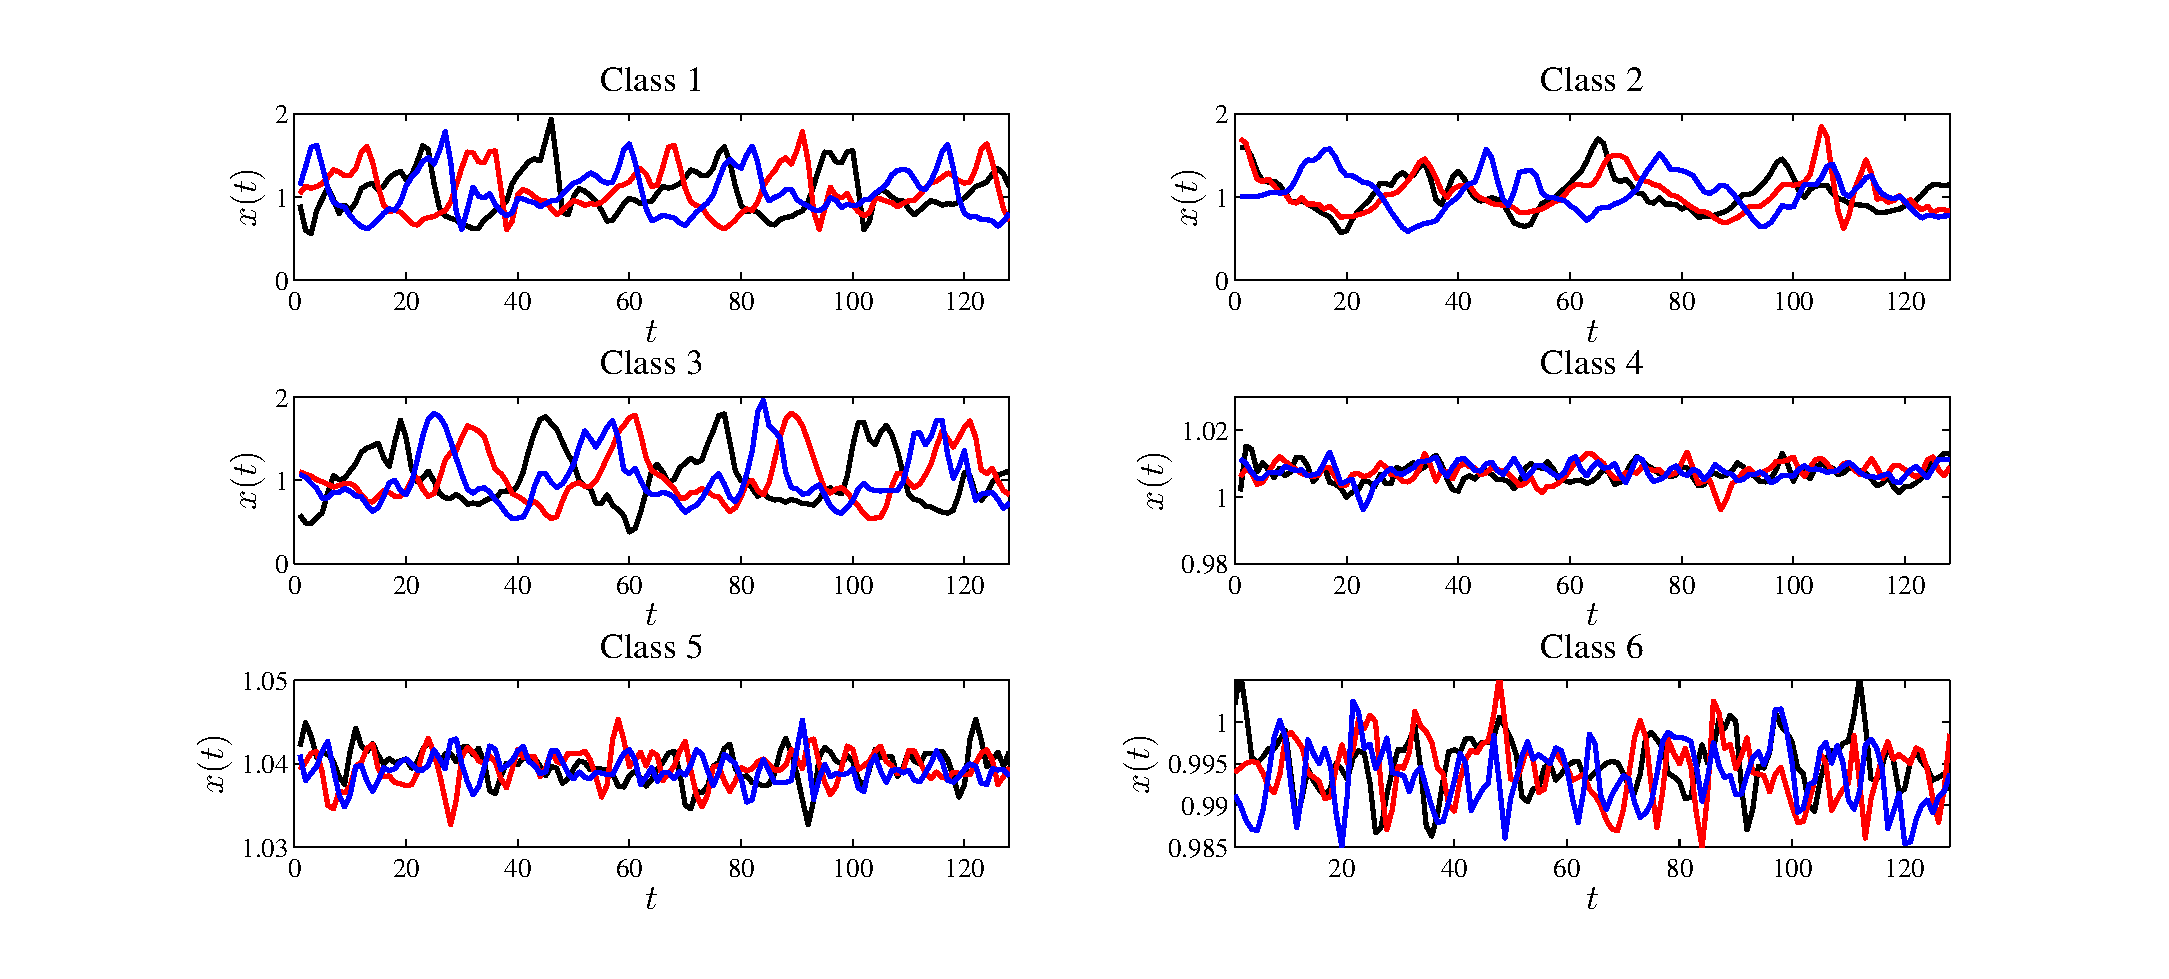
\includegraphics[width=1\linewidth]{figs/ch5/raw_ts}
		\caption{Примеры временных рядов акселерометра}
		\label{ch5:fig:raw_ts}
	\end{figure}
	\begin{figure}[!ht]
		\centering
		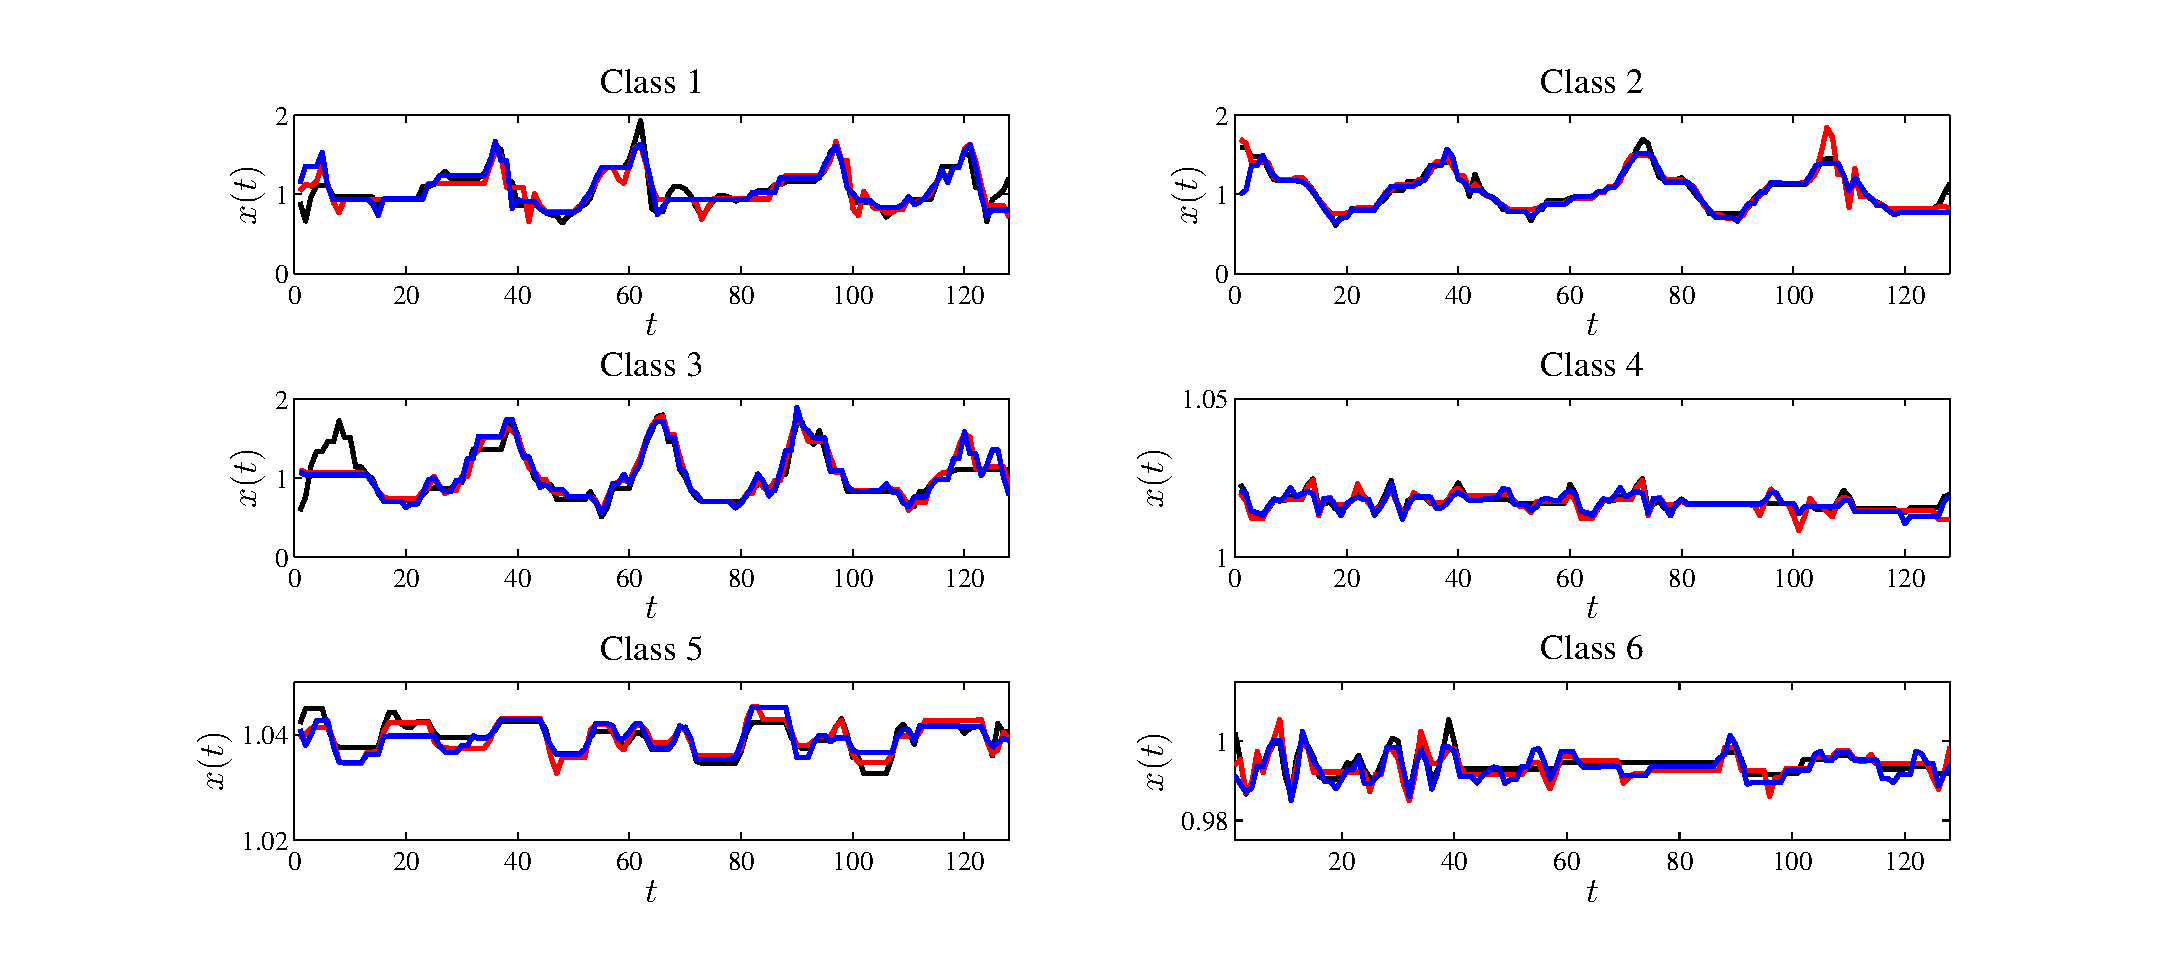
\includegraphics[width=1\linewidth]{figs/ch5/aligned_ts}
		\caption{Выравненные временные ряды акселерометра}
		\label{ch5:fig:aligned_ts}
	\end{figure}
	
	Ошибка классификации без использования метрического обучения составила~$37,5\%$.
	Алгоритм LMNN позволяет настроить параметры: число ближайших соседей~$k$,
	размерность преобразованного евклидова пространства~$p$.
	Для выбора оптимальных параметров воспользуемся процедурой кросс-валидации.
	На Рис.~\ref{ch5:fig:heat_map} цветом показана ошибка классификации алгоритма в зависимости от его параметров.
	На данной выборке алгоритм LMNN оказывается слабо чувствителен к числу ближайших соседей,
	и при уменьшении размерности пространства объектов ошибка классификации растет.
	\begin{figure}[!ht]
		\centering
		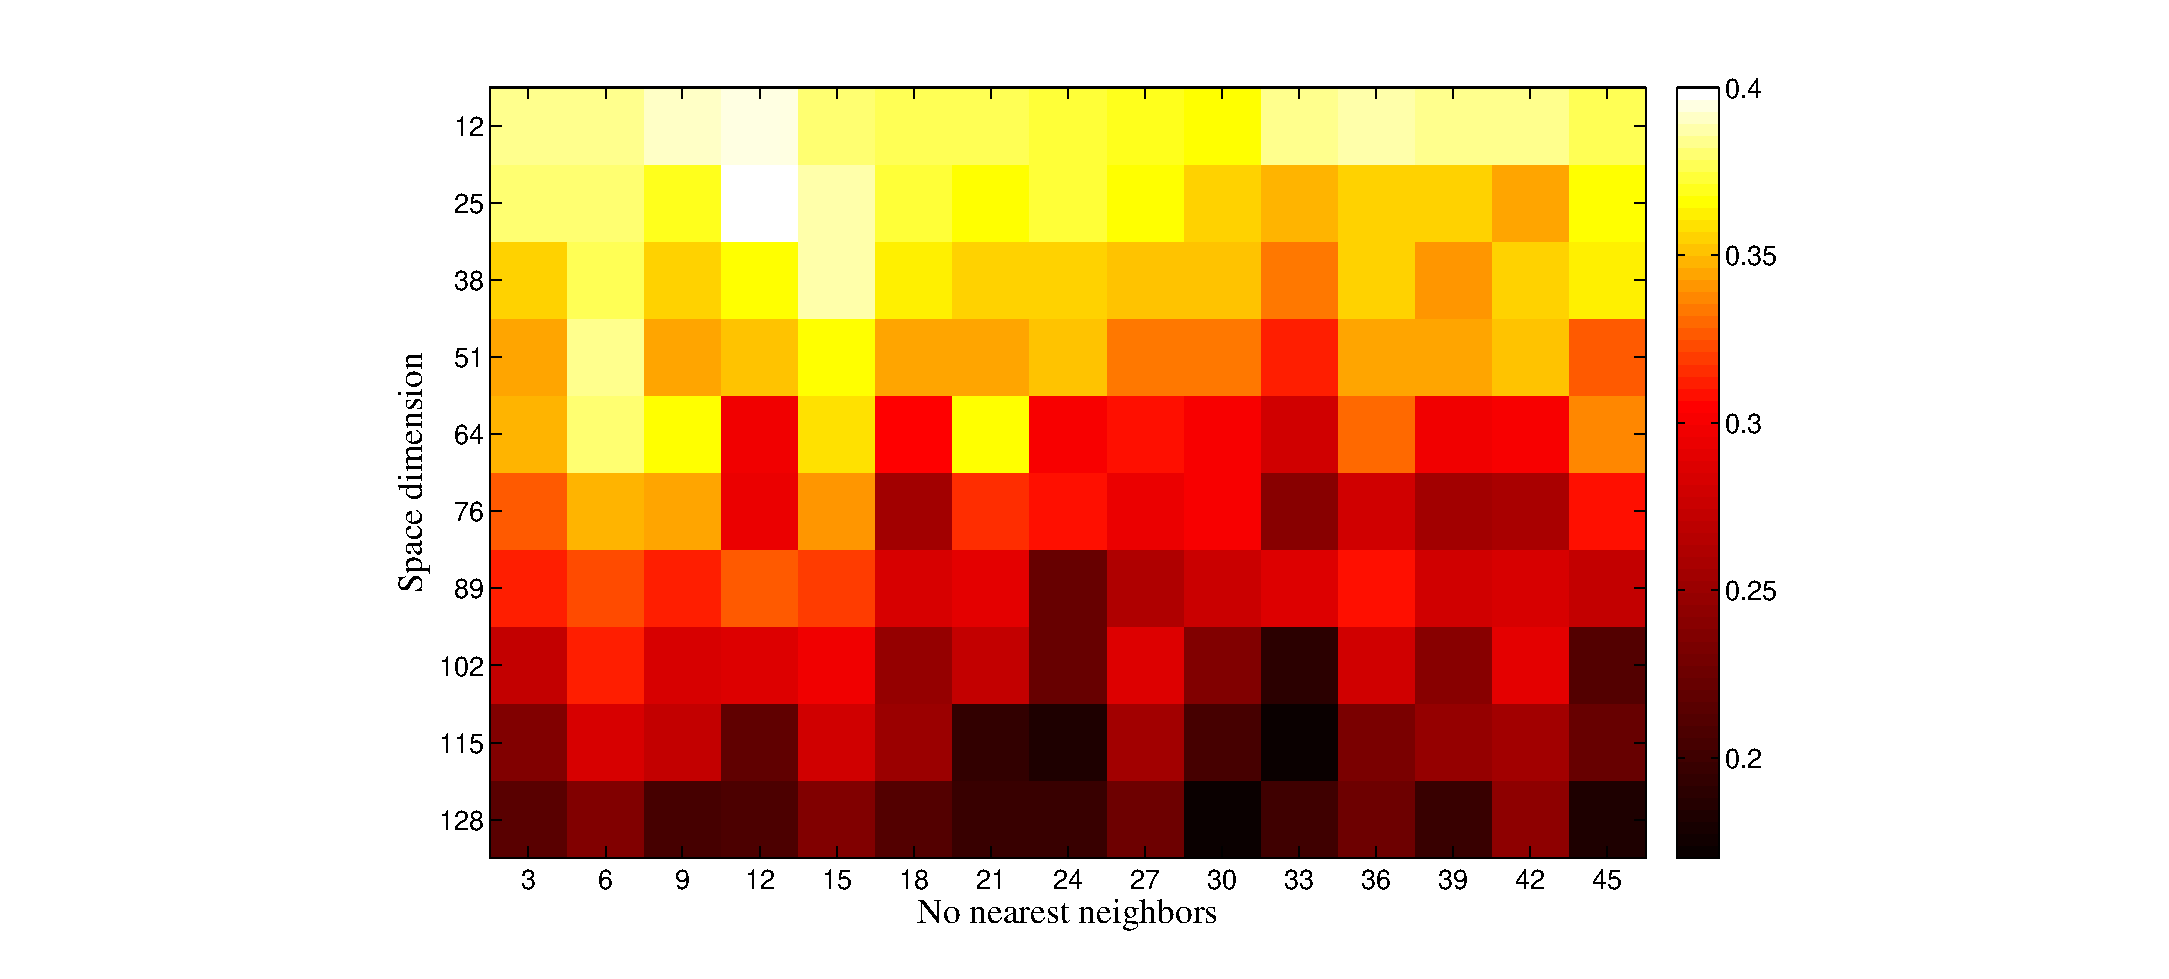
\includegraphics[width=1\linewidth]{figs/ch5/heat_map}
		\caption{Ошибка классификации метрического алгоритма в зависимости от размерности пространства и количества используемых ближайших соседей}
		\label{ch5:fig:heat_map}
	\end{figure}
	
	Настроим алгоритм LMNN со следующими параметрами: число ближайших соседей $k = 30$, размерность
	выходного пространства $p = 128$.
	Ошибка классификации составила~$17,25\%$, что вдвое меньше ошибки классификации с использованием евклидовой метрики.
	
	\begin{table}
		\centering
		\caption{Матрицы несоответствий для евклидовой метрики и метрики Махаланобиса, построенные для временных рядов аксселерометра}
		\subfloat[][Евклидова метрика]{\begin{tabular}{|l|l|l|l|l|l|l|}
				\hline
				\multirow{2}{*}{} & \multicolumn{6}{c|}{Истинные метки классов} \\ \cline{2-7}
				& 1     & 2     & 3     & 4     & 5    & 6    \\ \hline
				1                 & 80    & 0     & 5     & 0     & 0    & 0    \\ \hline
				2                 & 4     & 56    & 33    & 0     & 0    & 0    \\ \hline
				3                 & 5     & 5     & 86    & 0     & 0    & 0    \\ \hline
				4                 & 7     & 8     & 5     & 168   & 4    & 21   \\ \hline
				5                 & 51    & 61    & 57    & 12    & 192  & 11   \\ \hline
				6                 & 53    & 70    & 14    & 20    & 2    & 168  \\ \hline
		\end{tabular}}
		\qquad
		\subfloat[][Метрика Махаланобиса]{\begin{tabular}{|l|l|l|l|l|l|l|}
				\hline
				\multirow{2}{*}{} & \multicolumn{6}{c|}{Истинные метки классов} \\ \cline{2-7}
				& 1     & 2     & 3     & 4     & 5    & 6    \\ \hline
				1                 & 151   & 12    & 13    & 0     & 0    & 0    \\ \hline
				2                 & 10    & 142   & 14    & 0     & 0    & 0    \\ \hline
				3                 & 9     & 10    & 171   & 0     & 0    & 0    \\ \hline
				4                 & 10    & 7     & 0     & 173   & 9    & 21   \\ \hline
				5                 & 2     & 11    & 0     & 12    & 186  & 9    \\ \hline
				6                 & 18    & 18    & 2     & 15    & 5    & 170  \\ \hline
		\end{tabular}}
		\label{ch5:tbl:confussion_matrix}
	\end{table}
	
	В таблице~\ref{ch5:tbl:confussion_matrix} представлены матрицы несоответствий результатов классификации при использовании
	евклидовой метрики и метрики Махаланобиса.
	Столбцы соответствуют истинным меткам классов объектов, строки~--- предсказанным меткам.
	Диагональное преобладание матрицы несоответствий указывает на высокую предсказательную способность алгоритма.
	
	В таблице~\ref{ch5:tbl:improvement} продемонстрировано увеличение точности классификации при использовании в качестве меры расстояния метрики Махаланобиса.
	Пересечение $i$-го столбца и $j$-й строки отвечает изменению доли объектов класса $i$, отнесенных к классу $j$. Положительное суммарное значение диагональных элементов таблицы соответствует увеличению качества классификации. Значительное улучшение предсказания происходит при классификации первых трех классов.
	Данные классы соответствуют следующим видам физической активности: ходьба, ходьба вверх, ходьба вниз.
	
	\begin{table}
		\centering
		\caption{Прирост точности классификации при использовании адекватной оценки матрицы трансформаций}
		\label{ch5:tbl:improvement}
		\begin{tabular}{|l|l|l|l|l|l|l|}
			\hline
			\multirow{2}{*}{} & \multicolumn{6}{c|}{Истинные метки классов}       \\ \cline{2-7}
			& 1      & 2      & 3      & 4      & 5     & 6     \\ \hline
			1   & \textbf{0,355}  & 0,06   & 0,04   & 0      & 0     & 0     \\ \hline
			2   & 0,03   & \textbf{0,43}   & --0,095 & 0      & 0     & 0     \\ \hline
			3   & 0,02   & 0,025  & \textbf{0,425}  & 0      & 0     & 0     \\ \hline
			4   & 0,015  & --0,005 & --0,025 & \textbf{0,025}  & 0,025 & 0     \\ \hline
			5   & --0,245 & --0,25  & --0,28  & 0      & \textbf{--0,03} & --0,01 \\ \hline
			6   & --0,175 & --0,26  & --0,06  & --0,025 & 0,005 & \textbf{--0,01} \\ \hline
		\end{tabular}
	\end{table}
	